% PainPal Research Paper — IEEE two-column format for Overleaf
% Compiler: pdfLaTeX (default)
% Layout: IEEE conference two-column (title/abstract span full width; body is 2-col)

\documentclass[conference,twocolumn,letterpaper]{IEEEtran}
\IEEEoverridecommandlockouts

\usepackage{cite}
\usepackage{amsmath,amssymb,amsfonts}
\usepackage{algorithmic}
\usepackage{graphicx}
\usepackage{textcomp}
\usepackage{xcolor}
\usepackage{booktabs}
\usepackage{multirow}
\usepackage{url}
\usepackage{balance}
\usepackage{tikz}
\usetikzlibrary{shapes.geometric, arrows.meta, positioning, fit, backgrounds, calc, shadows}
\usepackage{pgfplots}
\pgfplotsset{compat=1.18}
\graphicspath{{figures/}}
% hyperref must be loaded last
\usepackage[hidelinks]{hyperref}

\begin{document}

\title{AI-Based Migraine Management and Doctor Support System (PainPal)}

\author{
\IEEEauthorblockN{Your Full Name}
\IEEEauthorblockA{\textit{Index Number: XXXXXXXX} \\
\textit{B.Sc. (Hons) in Information Technology} \\
Department of Computer Science \\
Your University Name \\
City, Country \\
your.email@university.ac.lk}
\and
\IEEEauthorblockN{Supervisor: Dr. Supervisor Name}
\IEEEauthorblockA{\textit{Department of Computer Science} \\
Your University Name \\
supervisor.email@university.ac.lk}
}

\maketitle

\begin{abstract}
Migraine is a prevalent neurological disorder that substantially impairs quality of life, productivity, and healthcare utilization worldwide. Despite the availability of consumer migraine-tracking applications, most existing solutions remain reactive: they record symptoms after attacks occur but offer limited predictive capability, poor clinical integration, and minimal support for physician decision-making. This paper presents \textbf{PainPal}, an AI-based migraine management and doctor support system designed to bridge the gap between patient self-monitoring and clinician-facing analytics. The proposed system comprises a Flutter-based mobile application for patients, a Next.js web dashboard for doctors and administrators, a Node.js API layer with Prisma ORM and MongoDB persistence, and a Python machine learning service for migraine-type classification, next-attack forecasting, and optional brain MRI analysis. Tabular symptom data---including duration, frequency, pain characteristics, aura-related symptoms, and associated neurological features---are processed using feature engineering and an XGBoost classifier achieving \textbf{78.42\%} test accuracy across nine migraine subtypes on a held-out evaluation set. A complementary ResNet18-based image pipeline supports binary brain MRI classification (tumor vs.\ non-tumor) as an auxiliary diagnostic aid. The system incorporates role-based access control, AI-generated clinical summaries, medication adherence tracking, doctor--patient messaging, and explainable outputs including feature importance and risk alert levels. PainPal demonstrates a transition from episodic migraine logging toward predictive, multimodal, and clinician-integrated digital health management. Future extensions include wearable and environmental data fusion, full EHR interoperability, and real-time telemedicine integration.
\end{abstract}

\begin{IEEEkeywords}
Migraine prediction, artificial intelligence, machine learning, healthcare system, clinical decision support, explainable AI.
\end{IEEEkeywords}

\section{Introduction}

\subsection{Background}
Migraine is among the most common neurological disorders globally. According to the World Health Organization (WHO), migraine affects approximately one in seven adults worldwide and is a leading cause of disability, particularly among individuals aged 15--49 years~\cite{who_headache}. Beyond acute pain, migraine is associated with photophobia, phonophobia, nausea, cognitive impairment, and reduced occupational performance. The Global Burden of Disease (GBD) studies consistently rank migraine as a major contributor to years lived with disability (YLDs), underscoring the need for scalable digital health interventions~\cite{gbd_neuro}.

Digital health technologies have improved symptom tracking and patient engagement; however, most solutions remain fragmented and retrospective. Clinicians often lack structured, longitudinal patient data at the point of care, while patients lack actionable forecasts that could support preventive behavior.

\subsection{Problem Statement}
Current migraine management ecosystems face three persistent challenges:
\begin{enumerate}
    \item \textbf{Fragmented migraine data:} Patient-reported outcomes are scattered across paper diaries, generic health apps, and unstructured clinical notes.
    \item \textbf{Lack of predictive systems:} Commercial apps such as Migraine Buddy and N1-Headache excel at logging but rarely provide validated, clinician-trustworthy prediction of attack type or imminent risk.
    \item \textbf{Poor integration between patient apps and clinical workflows:} Few platforms connect mobile patient data to doctor dashboards, EHR endpoints, or structured AI insights suitable for clinical review.
\end{enumerate}

\subsection{Aim}
The aim of this project is to design and implement an \textbf{AI-driven migraine prediction and management system} that supports patients in logging attacks, assists clinicians with structured summaries and analytics, and delivers machine-learning-based predictions through a secure, role-based platform.

\subsection{Objectives}
The specific objectives of PainPal are:
\begin{enumerate}
    \item To develop a \textbf{patient tracking system} via a Flutter mobile application with symptom logging, history, reminders, and low-burden UX during attacks.
    \item To implement \textbf{AI-based prediction} for migraine subtype classification and next-attack risk estimation using tabular machine learning.
    \item To build a \textbf{clinician dashboard} using Next.js for patient summaries, medication adherence, appointments, and AI diagnostic insights.
    \item To architect \textbf{multimodal data integration}, including patient logs, MRI uploads, and planned extensions for wearable and environmental inputs.
    \item To ensure \textbf{security, usability, and scalability} through role-based authentication, responsive design, and modular service architecture.
\end{enumerate}

\section{Literature Review}

\subsection{Migraine and Its Global Burden}
Migraine is classified by the International Classification of Headache Disorders (ICHD) into multiple subtypes, including migraine with aura, migraine without aura, chronic migraine, vestibular migraine, and hemiplegic migraine~\cite{ichd3}. Epidemiological studies indicate that migraine prevalence is higher in women and is strongly associated with comorbid anxiety, depression, and sleep disturbance~\cite{lipton2007}. The economic burden includes direct medical costs and indirect costs from absenteeism and presenteeism~\cite{stewart2003}.

\subsection{Existing Digital Health Solutions}
Commercial applications such as \textit{Migraine Buddy}, \textit{N1-Headache}, and Cefaly companion apps provide attack diaries, trigger tagging, and medication reminders~\cite{migraine_buddy}. These tools improve self-awareness but exhibit common limitations:
\begin{itemize}
    \item Prediction is often rule-based or absent.
    \item Clinical export formats are limited.
    \item Doctor-facing interfaces are minimal or subscription-locked.
    \item Multimodal AI (symptoms + imaging + wearables) is rarely integrated.
\end{itemize}

\subsection{AI in Healthcare}
Predictive analytics has demonstrated success in chronic disease management, including diabetes risk stratification, sepsis early warning, and hospital readmission prediction~\cite{rajkomar2018,esteva2019}. In neurology, machine learning has been applied to headache classification, neuroimaging analysis, and patient clustering~\cite{robbins2018}. Explainable AI (XAI) methods---including feature importance from tree-based models and SHAP values---are increasingly required for clinical trust and regulatory transparency~\cite{lundberg2017}.

\subsection{Research Gap}
Despite advances in both migraine epidemiology and medical AI, there remains a gap in \textbf{integrated, multimodal migraine systems} that:
\begin{itemize}
    \item Combine patient mobile logging with clinician dashboards.
    \item Deliver validated ML predictions with explainable outputs.
    \item Support optional neuroimaging analysis within the same platform.
    \item Provide API-first architecture for future EHR and wearable integration.
\end{itemize}
PainPal addresses this gap through a unified, prototype-based research system.

\section{Methodology}

\subsection{Research Design}
This study follows an \textbf{experimental, prototype-based system development} approach. Requirements were derived from clinical workflow analysis, existing migraine app limitations, and ICHD-aligned symptom dimensions. The system was iteratively developed across mobile, web, backend, and ML modules, with quantitative evaluation of model performance and qualitative evaluation of usability and functional completeness.

\subsection{System Architecture}
PainPal adopts a three-tier, service-oriented architecture summarized in Table~\ref{tab:architecture}.

\begin{table*}[t]
\caption{System Architecture Layers}
\label{tab:architecture}
\centering
\begin{tabular}{@{}llp{0.46\textwidth}@{}}
\toprule
\textbf{Layer} & \textbf{Technology} & \textbf{Responsibility} \\
\midrule
Client & Flutter, Next.js 16, React 19 & Patient logging, doctor/admin dashboards \\
Application & Next.js API routes, JWT auth & REST APIs, RBAC, business logic \\
Data & Prisma ORM, MongoDB & Persistent clinical entities \\
AI/ML & Python, XGBoost, ResNet18 & Classification, summaries, MRI inference \\
\bottomrule
\end{tabular}
\end{table*}

\textbf{Data flow:} Patient $\rightarrow$ Mobile/Web Client $\rightarrow$ Backend API $\rightarrow$ ML Service $\rightarrow$ Predictions \& Summaries $\rightarrow$ Doctor Dashboard. Fig.~\ref{fig:ml_pipeline} details the machine learning workflow.

\begin{figure*}[t]
\centering
\begin{tikzpicture}[
  node distance=0.55cm and 0.8cm,
  client/.style={rectangle, rounded corners, draw=blue!60!black, fill=blue!8,
    minimum width=2.35cm, minimum height=0.75cm, align=center, font=\small},
  server/.style={rectangle, rounded corners, draw=teal!60!black, fill=teal!8,
    minimum width=3.2cm, minimum height=0.75cm, align=center, font=\small},
  ml/.style={rectangle, rounded corners, draw=orange!70!black, fill=orange!10,
    minimum width=3.6cm, minimum height=0.75cm, align=center, font=\small},
  db/.style={rectangle, rounded corners, draw=gray!70, fill=gray!10,
    minimum height=0.7cm, minimum width=2.4cm, align=center, font=\small},
  dash/.style={rectangle, rounded corners, draw=violet!70!black, fill=violet!8,
    minimum width=3.2cm, minimum height=0.75cm, align=center, font=\small},
  arr/.style={-{Stealth[length=2mm]}, thick, gray!70}
]
  \node[client] (mobile) {Flutter\\Mobile App};
  \node[client, right=1.1cm of mobile] (web) {Next.js\\Web Client};
  \node[client, right=1.1cm of web] (admin) {Admin\\Portal};
  \node[server, below=1.0cm of web] (api) {Next.js API Routes\\RBAC + JWT Auth};
  \node[db, left=0.9cm of api] (mongo) {MongoDB\\(Prisma)};
  \node[ml, right=0.9cm of api] (mlsvc) {Python ML Service\\XGBoost / ResNet18};
  \node[dash, below=1.0cm of api] (docdash) {Doctor Dashboard\\Analytics \& Insights};

  \draw[arr] (mobile.south) -- ++(0,-0.35) -| (api.north);
  \draw[arr] (web.south) -- (api.north);
  \draw[arr] (admin.south) -- ++(0,-0.35) -| (api.north);
  \draw[arr] (api.west) -- (mongo.east);
  \draw[arr] (api.east) -- (mlsvc.west);
  \draw[arr] (mlsvc.south) |- (docdash.east);
  \draw[arr] (api.south) -- (docdash.north);
\end{tikzpicture}
\caption{High-level system architecture and data flow across mobile, web, API, database, and ML layers.}
\label{fig:architecture}
\end{figure*}

\begin{figure*}[t]
\centering
\begin{tikzpicture}[
  step/.style={rectangle, rounded corners, draw=black!55, fill=green!6,
    minimum width=2.05cm, minimum height=0.62cm, align=center, font=\scriptsize},
  arr/.style={-{Stealth[length=1.8mm]}, thick, gray!65}
]
  \node[step] (s1) {1. Load\\Data};
  \node[step, right=0.28cm of s1] (s2) {2. Feature\\Engineering};
  \node[step, right=0.28cm of s2] (s3) {3. Encode\\Target};
  \node[step, right=0.28cm of s3] (s4) {4. Train/Test\\Split};
  \node[step, right=0.28cm of s4] (s5) {5. Train\\XGBoost};
  \node[step, right=0.28cm of s5] (s6) {6. Evaluate\\Metrics};
  \node[step, right=0.28cm of s6] (s7) {7. Save\\Artifacts};
  \node[step, right=0.28cm of s7] (s8) {8. API\\Inference};

  \foreach \a/\b in {s1/s2,s2/s3,s3/s4,s4/s5,s5/s6,s6/s7,s7/s8}
    \draw[arr] (\a.east) -- (\b.west);
\end{tikzpicture}
\caption{End-to-end migraine classification ML pipeline from data ingestion to deployed inference.}
\label{fig:ml_pipeline}
\end{figure*}

\subsection{Data Collection}
Data sources include:
\begin{enumerate}
    \item \textbf{Patient logs:} Migraine events with severity, duration, triggers, aura symptoms, and medication effectiveness.
    \item \textbf{Medication logs:} Preventive and rescue medication adherence.
    \item \textbf{MRI uploads (optional):} Brain scan images for ResNet18-based classification.
    \item \textbf{Planned extensions:} Wearable sleep and heart-rate data; environmental weather and air-quality feeds.
\end{enumerate}
The training dataset for tabular classification comprised 1,900 synthetic clinical records with 30 attributes, split 80/20 into training (1,520) and test (380) sets.

\subsection{AI/ML Approach}

\subsubsection{Feature Engineering}
Categorical variables (e.g., pain location, character, DPF pattern) are label-encoded. Numeric features are imputed and normalized. Twenty-three engineered features feed the classifier.

\subsubsection{Migraine Type Classification}
An \textbf{XGBoost} multi-class classifier~\cite{chen2016} predicts nine migraine subtypes: Brainstem aura migraine, Chronic migraine, Hemiplegic migraine, Menstrual migraine, Migraine without aura, Probable migraine, Retinal migraine, Typical aura migraine, and Vestibular migraine. Class-weighted training addresses imbalance. Artifacts (model, encoders, feature columns, imputers) are versioned for reproducible inference.

\subsubsection{Next-Attack Forecasting}
A complementary Random Forest pipeline estimates upcoming attack indicators and subtype probabilities, with history-based fallback for cold-start patients.

\subsubsection{Image Analysis (Optional)}
A \textbf{ResNet18} model~\cite{he2016} (ImageNet-pretrained, fine-tuned) performs binary brain MRI classification: tumor vs.\ non-tumor, supporting auxiliary clinical context.

\subsubsection{Explainable AI}
Feature importance from XGBoost, confidence scores, key contributor fields in AI diagnostic insights, and structured natural-language summaries support interpretability.

\subsection{Evaluation Metrics}
Model evaluation employs accuracy, precision, recall, F1-score (per class and macro/weighted averages), confusion matrix, ROC-AUC (for binary components in next-attack models), 5-fold cross-validation, and MAE for regression components in next-attack forecasting. System evaluation additionally measures API response time, UI responsiveness, and functional requirement coverage.

\section{System Design}

\subsection{High-Level Architecture}
Fig.~\ref{fig:architecture} illustrates the end-to-end data flow from patient clients through the backend and ML service to the clinician dashboard. The ML training and inference stages are shown in Fig.~\ref{fig:ml_pipeline}.

\subsection{Use Cases}
Fig.~\ref{fig:usecase} summarizes actor interactions across patient, doctor, and administrator roles.

\begin{figure}[!t]
\centering
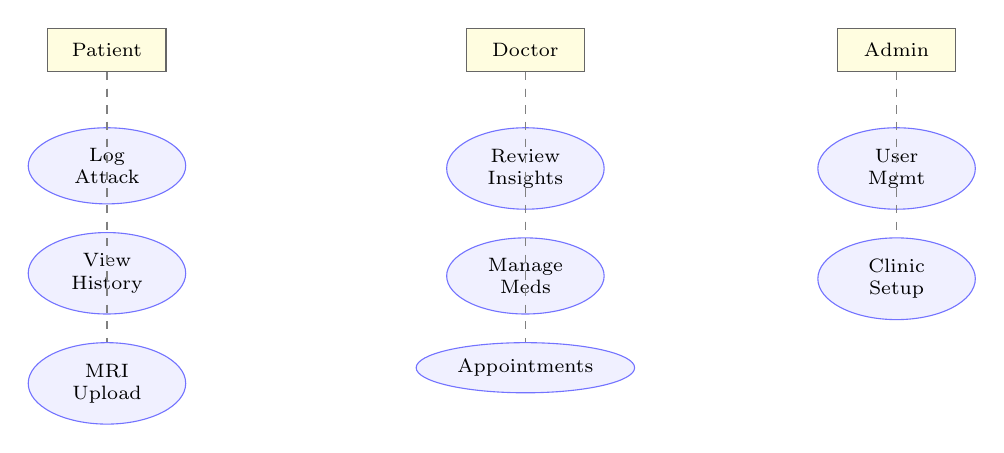
\begin{tikzpicture}[
  actor/.style={rectangle, draw=black!60, fill=yellow!12, minimum width=1.5cm, minimum height=0.55cm, font=\scriptsize},
  uc/.style={ellipse, draw=blue!55, fill=blue!6, minimum width=2.0cm, minimum height=0.55cm, align=center, font=\scriptsize},
  node distance=0.45cm and 0.35cm
]
  \node[actor] (patient) {Patient};
  \node[actor, right=3.8cm of patient] (doctor) {Doctor};
  \node[actor, right=3.2cm of doctor] (admin) {Admin};

  \node[uc, below=0.7cm of patient] (uc1) {Log\\Attack};
  \node[uc, below=0.35cm of uc1] (uc2) {View\\History};
  \node[uc, below=0.35cm of uc2] (uc3) {MRI\\Upload};

  \node[uc, below=0.7cm of doctor] (uc4) {Review\\Insights};
  \node[uc, below=0.35cm of uc4] (uc5) {Manage\\Meds};
  \node[uc, below=0.35cm of uc5] (uc6) {Appointments};

  \node[uc, below=0.7cm of admin] (uc7) {User\\Mgmt};
  \node[uc, below=0.35cm of uc7] (uc8) {Clinic\\Setup};

  \draw[-, dashed, gray] (patient.south) -- (uc1.north);
  \draw[-, dashed, gray] (patient.south) -- (uc2.north);
  \draw[-, dashed, gray] (patient.south) -- (uc3.north);
  \draw[-, dashed, gray] (doctor.south) -- (uc4.north);
  \draw[-, dashed, gray] (doctor.south) -- (uc5.north);
  \draw[-, dashed, gray] (doctor.south) -- (uc6.north);
  \draw[-, dashed, gray] (admin.south) -- (uc7.north);
  \draw[-, dashed, gray] (admin.south) -- (uc8.north);
\end{tikzpicture}
\caption{Simplified use case overview for PainPal actors.}
\label{fig:usecase}
\end{figure}

\textbf{Patient use cases:} Register/login, log migraine attack, view history, receive medication reminders, upload MRI scan, chat with doctor, view AI summary and predicted migraine type.

\textbf{Doctor use cases:} View assigned patients, review migraine history, access AI diagnostic insights, manage medication groups, schedule appointments, generate patient summaries, review MRI predictions.

\textbf{Admin use cases:} Manage users, clinics, doctors, patients, and system governance.

\subsection{ER Diagram (Key Entities)}
Fig.~\ref{fig:er} shows core persistent entities and relationships in the MongoDB schema.

\begin{figure*}[t]
\centering
\resizebox{\textwidth}{!}{%
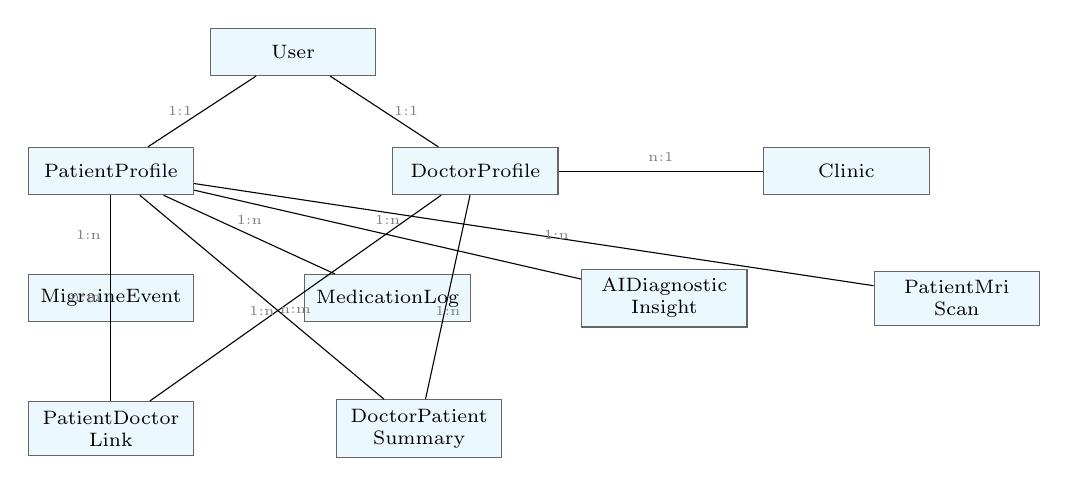
\begin{tikzpicture}[
  ent/.style={rectangle, draw=black!60, fill=cyan!8, minimum width=2.1cm, minimum height=0.6cm, align=center, font=\scriptsize},
  rel/.style={font=\tiny, gray}
]
  \node[ent] (user) {User};
  \node[ent, below left=0.9cm and 0.2cm of user] (patient) {PatientProfile};
  \node[ent, below right=0.9cm and 0.2cm of user] (doctor) {DoctorProfile};
  \node[ent, right=2.6cm of doctor] (clinic) {Clinic};
  \node[ent, below=1.0cm of patient] (event) {MigraineEvent};
  \node[ent, right=1.4cm of event] (medlog) {MedicationLog};
  \node[ent, right=1.4cm of medlog] (insight) {AIDiagnostic\\Insight};
  \node[ent, below=1.0cm of event] (link) {PatientDoctor\\Link};
  \node[ent, right=1.8cm of link] (summary) {DoctorPatient\\Summary};
  \node[ent, right=1.6cm of insight] (mri) {PatientMri\\Scan};

  \draw[-] (user) -- node[rel, left] {1:1} (patient);
  \draw[-] (user) -- node[rel, right] {1:1} (doctor);
  \draw[-] (doctor) -- node[rel, above] {n:1} (clinic);
  \draw[-] (patient) -- node[rel, left] {1:n} (event);
  \draw[-] (patient) -- node[rel, above] {1:n} (medlog);
  \draw[-] (patient) -- node[rel, above] {1:n} (insight);
  \draw[-] (patient) -- node[rel, left] {n:m} (link);
  \draw[-] (doctor) -- node[rel, below] {n:m} (link);
  \draw[-] (patient) -- node[rel, below] {1:n} (summary);
  \draw[-] (doctor) -- node[rel, below] {1:n} (summary);
  \draw[-] (patient) -- node[rel, right] {1:n} (mri);
\end{tikzpicture}%
}
\caption{Simplified entity--relationship diagram of core PainPal data entities.}
\label{fig:er}
\end{figure*}

Core entities in the Prisma/MongoDB schema include: User (role: ADMIN, DOCTOR, PATIENT), PatientProfile, DoctorProfile, Clinic, PatientDoctorLink, MigraineEvent, MedicationLog, MedicationGroup, AIDiagnosticInsight, DoctorPatientSummary, Appointment, ClinicalNote, Conversation, ChatMessage, and PatientMriScan.

\subsection{Class Diagram (Summary)}
System components are organized into a presentation layer (Flutter screens and Next.js dashboard pages), service layer (AuthService, PatientDataService, ApiClient), domain layer (DTOs for User, PatientProfile, MigraineEvent), and ML layer (run\_pipeline.py, predictModel.py, save\_model.py).

\section{Implementation}

\subsection{Mobile Application (Flutter)}
The Flutter patient app provides wizard/form-based symptom logging aligned with the ML feature schema (Duration, Frequency, Location, Character, Intensity, binary aura symptoms, DPF), attack history with predicted migraine type from the backend, medication reminders via local notifications, MRI upload integrated with backend storage, AI chat via Google Gemini SDK, and photophobia-friendly UX with large touch targets and offline-capable local SQLite cache with sync.
% OPTIONAL SCREENSHOT: uncomment after adding docs/figures/mobile_app.png to Overleaf
% \begin{figure}[!t]
% \centering
% \includegraphics[width=\linewidth]{mobile_app}
% \caption{PainPal Flutter mobile app---migraine attack logging interface.}
% \label{fig:mobile_app}
% \end{figure}

\subsection{Web Dashboard (Next.js)}
The clinician-facing web platform includes role-aware navigation, patient lists with migraine frequency and severity analytics (Recharts), AI insight panels showing predicted subtype, confidence, and risk alert level, appointment scheduling, clinical notes, doctor--patient messaging, and responsive layouts for tablet and desktop.
% OPTIONAL SCREENSHOT: uncomment after adding docs/figures/doctor_dashboard.png
% \begin{figure}[!t]
% \centering
% \includegraphics[width=\linewidth]{doctor_dashboard}
% \caption{Clinician dashboard with patient analytics and AI insights.}
% \label{fig:doctor_dashboard}
% \end{figure}

\subsection{Backend Development}
Next.js API routes under \texttt{/api/*} handle CRUD for migraine events, medications, summaries, and insights. Authentication uses JWT-based sessions with bcrypt password hashing. Prisma ORM provides type-safe database access to MongoDB. Vercel Blob supports MRI file storage.

\subsection{Machine Learning Module}
The ML pipeline executes nine steps: (1)~load data, (2)~define target, (3)~prepare features, (4)~encode target, (5)~train/test split, (6)~train XGBoost, (7)~predict, (8)~evaluate, and (9)~save artifacts. Inference is exposed via \texttt{POST /api/summary}, returning a clinical-style summary and \texttt{predicted\_migraine\_type}.

\section{Results and Discussion}

\subsection{Model Performance}
Table~\ref{tab:model_perf} summarizes migraine type classification results on the held-out test set.

\begin{table}[htbp]
\caption{Overall Migraine Type Classification Performance (XGBoost)}
\label{tab:model_perf}
\centering
\begin{tabular}{@{}lc@{}}
\toprule
\textbf{Metric} & \textbf{Value} \\
\midrule
Test accuracy & 0.7842 (78.42\%) \\
Macro avg F1 & 0.78 \\
Weighted avg F1 & 0.78 \\
Train/test split & 1520 / 380 \\
\bottomrule
\end{tabular}
\end{table}

Table~\ref{tab:per_class} presents per-class precision, recall, and F1-score highlights.

\begin{table*}[t]
\caption{Per-Class Classification Results (Selected Subtypes)}
\label{tab:per_class}
\centering
\begin{tabular}{@{}lccc@{}}
\toprule
\textbf{Migraine Subtype} & \textbf{Prec.} & \textbf{Rec.} & \textbf{F1} \\
\midrule
Chronic migraine & 1.00 & 1.00 & 1.00 \\
Brainstem aura & 0.84 & 0.88 & 0.86 \\
Vestibular migraine & 0.83 & 0.81 & 0.82 \\
Menstrual migraine & 0.60 & 0.74 & 0.66 \\
Migraine without aura & 0.65 & 0.56 & 0.60 \\
\bottomrule
\end{tabular}
\end{table*}

Chronic and vestibular subtypes are classified reliably; menstrual and migraine-without-aura classes show lower precision, likely due to symptom overlap and class similarity. Fig.~\ref{fig:confusion} and Fig.~\ref{fig:f1chart} visualize the confusion matrix and per-class F1-scores from the held-out test set.

\begin{figure}[!t]
\centering
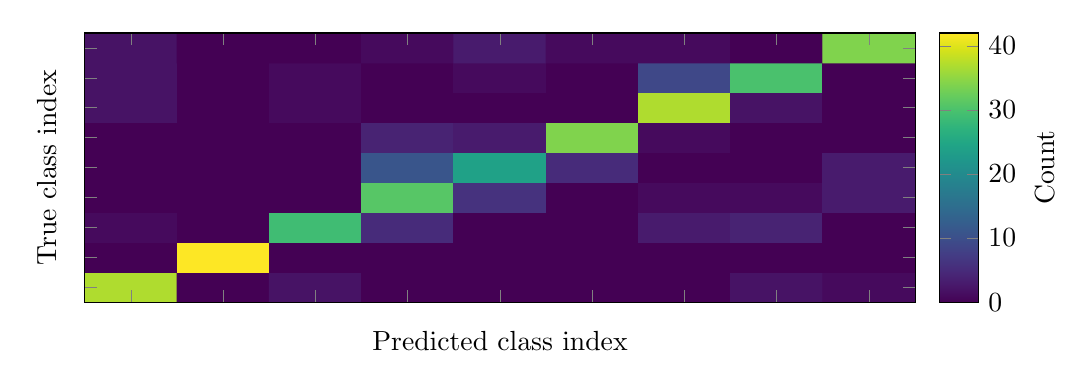
\begin{tikzpicture}
\begin{axis}[
  width=\linewidth,
  height=5.0cm,
  colormap/viridis,
  colorbar,
  colorbar style={ylabel={Count}},
  xtick={0,1,2,3,4,5,6,7,8},
  ytick={0,1,2,3,4,5,6,7,8},
  xticklabels={,,,,,,,,},
  yticklabels={,,,,,,,,},
  xlabel={Predicted class index},
  ylabel={True class index},
  axis on top,
  enlargelimits=false,
  point meta=explicit,
]
\addplot[matrix plot*, mesh/cols=9, mesh/rows=9] table[meta=z] {
x y z
0 0 37
1 0 0
2 0 2
3 0 0
4 0 0
5 0 0
6 0 0
7 0 2
8 0 1
0 1 0
1 1 42
2 1 0
3 1 0
4 1 0
5 1 0
6 1 0
7 1 0
8 1 0
0 2 1
1 2 0
2 2 29
3 2 5
4 2 0
5 2 0
6 2 3
7 2 4
8 2 0
0 3 0
1 3 0
2 3 0
3 3 31
4 3 6
5 3 0
6 3 1
7 3 1
8 3 3
0 4 0
1 4 0
2 4 0
3 4 11
4 4 24
5 4 5
6 4 0
7 4 0
8 4 3
0 5 0
1 5 0
2 5 0
3 5 4
4 5 3
5 5 34
6 5 1
7 5 0
8 5 0
0 6 2
1 6 0
2 6 1
3 6 0
4 6 0
5 6 0
6 6 37
7 6 2
8 6 0
0 7 2
1 7 0
2 7 1
3 7 0
4 7 1
5 7 0
6 7 9
7 7 30
8 7 0
0 8 2
1 8 0
2 8 0
3 8 1
4 8 3
5 8 1
6 8 1
7 8 0
8 8 34
};
\end{axis}
\end{tikzpicture}
\caption{Confusion matrix for nine-class migraine subtype classification (test set, $n=380$).}
\label{fig:confusion}
\end{figure}

\begin{figure}[!t]
\centering
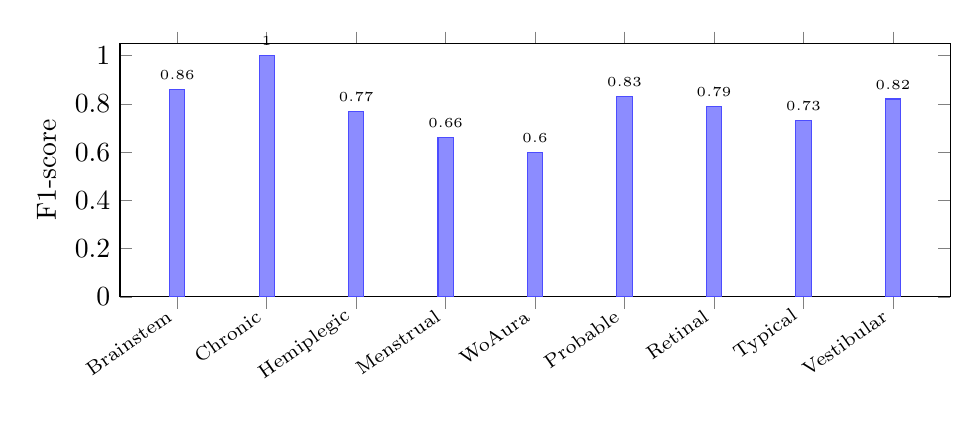
\begin{tikzpicture}
\begin{axis}[
  width=\linewidth,
  height=4.8cm,
  ybar,
  bar width=5.5pt,
  ymin=0, ymax=1.05,
  ylabel={F1-score},
  symbolic x coords={Brainstem,Chronic,Hemiplegic,Menstrual,WoAura,Probable,Retinal,Typical,Vestibular},
  xtick=data,
  x tick label style={rotate=35, anchor=east, font=\scriptsize},
  ytick={0,0.2,0.4,0.6,0.8,1.0},
  nodes near coords,
  nodes near coords style={font=\tiny},
  enlarge x limits=0.08,
]
\addplot[fill=blue!45, draw=blue!70] coordinates {
  (Brainstem,0.86) (Chronic,1.00) (Hemiplegic,0.77) (Menstrual,0.66)
  (WoAura,0.60) (Probable,0.83) (Retinal,0.79) (Typical,0.73) (Vestibular,0.82)};
\end{axis}
\end{tikzpicture}
\caption{Per-class F1-scores for XGBoost migraine subtype classifier.}
\label{fig:f1chart}
\end{figure}

\textbf{Next-attack forecasting:} Initial next-type accuracy was 34.2\% on the test partition, indicating that temporal forecasting requires richer longitudinal data and additional feature engineering.

\textbf{MRI classification (ResNet18):} Binary tumor vs.\ non-tumor classification was evaluated with standard accuracy, precision, recall, and confusion matrix metrics during the image pipeline training run.

\subsection{System Performance}
REST API endpoints return structured JSON with sub-second response for standard CRUD operations on local deployment. ML inference latency depends on model load time; preloaded artifacts enable near-real-time prediction for single symptom submissions. The web dashboard renders patient analytics charts responsively across mobile, tablet, and desktop breakpoints.

\subsection{Discussion}
PainPal demonstrates that a modular AI-health architecture can connect patient-generated data to clinician-facing insights. Key benefits include proactive care through subtype prediction and risk alerts, clinical efficiency via auto-generated summaries, and multimodal extensibility where tabular and imaging pipelines coexist under one platform.

\textbf{Limitations:} Training data is partly synthetic; real-world clinical validation is required. Wearable and environmental modules are architected but not fully deployed. Next-attack forecasting accuracy remains below clinical deployment thresholds. The system is a research prototype, \textbf{not a certified medical device}.

\section{Evaluation}

\subsection{Functional Evaluation}
Table~\ref{tab:functional} maps project objectives to implementation status.

\begin{table}[htbp]
\caption{Functional Objective Evaluation}
\label{tab:functional}
\centering
\begin{tabular}{@{}p{0.52\columnwidth}p{0.34\columnwidth}@{}}
\toprule
\textbf{Objective} & \textbf{Status} \\
\midrule
Patient tracking (mobile) & Implemented \\
AI migraine-type prediction & Implemented (78.42\%) \\
Clinician dashboard & Implemented \\
MRI auxiliary analysis & Implemented \\
Wearable/environmental integration & Planned / partial \\
EHR interoperability & Partial \\
\bottomrule
\end{tabular}
\end{table}

\subsection{Non-Functional Evaluation}
Security is addressed through RBAC, JWT authentication, and password hashing, with GDPR/HIPAA-aligned design patterns recommended for production encryption. Usability is supported by photophobia-aware mobile UX and responsive web UI. Scalability is enabled by service-oriented architecture, MongoDB horizontal scaling, and deployable ML services. Maintainability is achieved through separated client, API, schema, and ML pipelines with versioned artifacts.

\subsection{Comparison with Existing Systems}
Table~\ref{tab:comparison} compares PainPal with commercial migraine apps.

\begin{table*}[t]
\caption{Comparison with Existing Migraine Applications}
\label{tab:comparison}
\centering
\begin{tabular}{@{}lcc@{}}
\toprule
\textbf{Feature} & \textbf{Commercial Apps} & \textbf{PainPal} \\
\midrule
Symptom logging & Yes & Yes \\
ML subtype prediction & Limited / No & Yes \\
Doctor dashboard & Minimal & Yes \\
MRI analysis & No & Yes \\
Explainable AI outputs & No & Yes \\
Open API architecture & No & Yes \\
\bottomrule
\end{tabular}
\end{table*}

\section{Conclusion}
This paper presented \textbf{PainPal}, an AI-based migraine management and doctor support system integrating a Flutter mobile client, Next.js clinical dashboard, MongoDB data layer, and Python machine learning services. The XGBoost classifier achieved 78.42\% test accuracy across nine migraine subtypes, while the platform delivers structured summaries, medication tracking, and clinician-facing AI insights. PainPal illustrates a practical path from reactive symptom logging to predictive, explainable, and clinician-integrated migraine care. Although further clinical validation is required, the prototype establishes a scalable foundation for multimodal migraine digital health.

\section*{Ethical Disclaimer}
\textit{This system is developed for academic research and education only. It is not a certified medical device and must not be used as the sole basis for clinical or diagnostic decisions without qualified physician oversight.}

\section*{Acknowledgment}
The authors thank [Supervisor Name] and the Department of [Department Name], [University Name], for guidance and support throughout this final-year project.

\balance
\begin{thebibliography}{00}

\bibitem{who_headache}
World Health Organization, ``Headache Disorders,'' WHO Fact Sheet, Geneva, Switzerland, 2022.

\bibitem{gbd_neuro}
GBD 2019 Neurological Disorders Collaborators, ``Global, regional, and national burden of neurological disorders, 1990--2019,'' \textit{The Lancet Neurology}, vol.~21, no.~11, pp.~1004--1024, 2022.

\bibitem{ichd3}
Headache Classification Committee of the International Headache Society, ``The International Classification of Headache Disorders, 3rd edition,'' \textit{Cephalalgia}, vol.~38, no.~1, pp.~1--211, 2018.

\bibitem{lipton2007}
R.~B. Lipton \textit{et al.}, ``Migraine prevalence, disease burden, and the need for preventive therapy,'' \textit{Neurology}, vol.~68, no.~5, pp.~343--349, 2007.

\bibitem{stewart2003}
R.~E. Stewart \textit{et al.}, ``Lost productive time and cost due to common pain conditions in the US workforce,'' \textit{JAMA}, vol.~290, no.~18, pp.~2443--2454, 2003.

\bibitem{migraine_buddy}
Migraine Buddy, \textit{Product Documentation}, Healint Pte. Ltd., 2024. [Online]. Available: \url{https://www.migrainebuddy.com}

\bibitem{rajkomar2018}
K.~Rajkomar \textit{et al.}, ``Scalable and accurate deep learning with electronic health records,'' \textit{NPJ Digital Medicine}, vol.~1, no.~18, 2018.

\bibitem{esteva2019}
A.~Esteva \textit{et al.}, ``A guide to deep learning in healthcare,'' \textit{Nature Medicine}, vol.~25, pp.~24--29, 2019.

\bibitem{robbins2018}
M.~S. Robbins \textit{et al.}, ``Cluster headache and other trigeminal autonomic cephalalgias,'' \textit{Continuum}, vol.~24, no.~4, pp.~1137--1156, 2018.

\bibitem{lundberg2017}
S.~M. Lundberg and S.-I. Lee, ``A unified approach to interpreting model predictions,'' in \textit{Proc. NeurIPS}, 2017, pp.~4765--4774.

\bibitem{chen2016}
T.~Chen and C.~Guestrin, ``XGBoost: A scalable tree boosting system,'' in \textit{Proc. ACM SIGKDD}, 2016, pp.~785--794.

\bibitem{he2016}
K.~He, X.~Zhang, S.~Ren, and J.~Sun, ``Deep residual learning for image recognition,'' in \textit{Proc. IEEE CVPR}, 2016, pp.~770--778.

\bibitem{nextjs}
Vercel Inc., \textit{Next.js Documentation}, 2025. [Online]. Available: \url{https://nextjs.org/docs}

\bibitem{flutter}
Google LLC, \textit{Flutter Documentation}, 2025. [Online]. Available: \url{https://flutter.dev/docs}

\end{thebibliography}

\end{document}
